% This is not necessarily in the format for a VUW thesis chapter.

% Finished August 26, 2013

\documentclass[a4paper]{report}

\usepackage{amssymb, amsmath}
%\usepackage{mathtools}
\usepackage{tikz}
\usetikzlibrary{calc}

%\usepackage{marvosym}

\newcommand{\beff}{\ensuremath{b_{\mathrm{eff}}}}
\newcommand{\bmin}{\ensuremath{b_{\mathrm{min}}}}
\newcommand{\bmax}{\ensuremath{b_{\mathrm{max}}}}

\title{Chapter 5: The Perturbative Slip Length}
\author{Nat Lund}


\begin{document}
\maketitle

We derived an expression for the effective slip length using the homogenization technique; this is presented in the previous chapter.  However, prior to doing this, we derived an expression for the effective slip length using a different technique -- the method of perturbation.  The homogenized expression for $\beff$ holds for a non-flat surface, while the perturbative expression assumes a flat surface.  Thus, the homogenized $\beff$ subsumes the perturbative $\beff$ as a special case.  The derivation of $\beff$ by perturbation methods is presented here.

\vspace{1em}

We model the fluid system as incompressible, Stokes `creeping' flow, with velocity vector $\vec{u} = (u,v,w)$: 
\begin{gather}
\nabla^2 \vec{u} = \frac{1}{\mu} \nabla p  \\
\nabla \cdot \vec{u} = 0
\end{gather}

The bottom solid surface is modeled as the $z=0$ plane.  
The surface is \textbf{flat,} so simple Navier slip holds:
\begin{gather}
u(0) = b(x,y) \frac{\partial u}{\partial z} \rvert_{z=0}
\end{gather}

The intrinsic slip length of the surface $b(x,y)$ is a rectangular-periodic function, with period $L$ in the $x$ direction.
Flow is generally in the $x$ direction, driven by shear \emph{only.}  Therefore there is no pressure gradient, and the pressure has the same $x$-periodicity as the surface:
\begin{equation}
p(x,y,z) = p(x+L,y,z)
\end{equation}


Note that the Navier slip condition is scalar, while the bulk conditions are vector equations.  This is because only the $x$ velocity slip effect is relevant to our analysis.



\subsubsection*{Plug Flow}

Our method is to perturb the exact case of plug flow.  If fluid is shear-driven by a constant velocity plate at the top boundary, and experiences \textbf{perfect slip} at the bottom boundary:
\begin{gather}
u(x,y,\mathrm{top}) = u_d \text{  (constant)} \\
\frac{\partial u}{\partial z} \rvert_{z=0} = 0
\end{gather}
then the fluid has no resistance at the bottom, so the entire bulk quickly accelerates up to velocity of the driving plate.  So fluid flows as a \textbf{plug} of fluid all at the same velocity.

\begin{center}
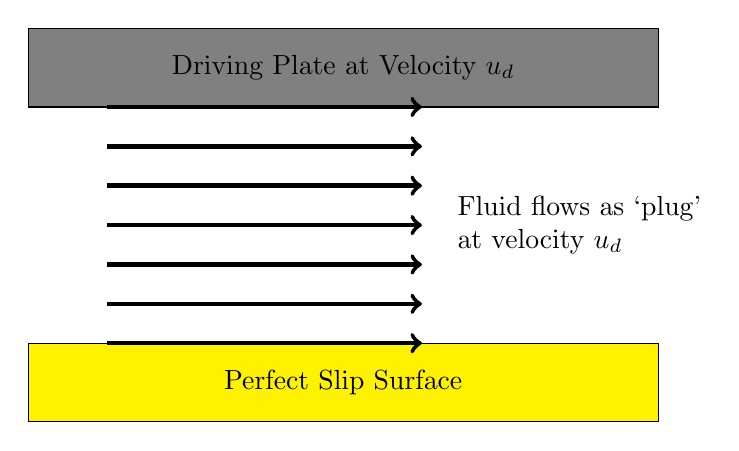
\begin{tikzpicture}
\draw[fill=yellow] (0,0) rectangle node{Perfect Slip Surface} (8,-1);
\draw[fill=gray] (0,3) rectangle node{Driving Plate at Velocity $u_d$} ++(8,1);

\foreach \z in {0,0.5,1,1.5,2,2.5,3}
    {\draw[->, ultra thick] (1,\z) -- ++(4,0);}
    
\node at (7,1.5)[align=left] {Fluid flows as `plug'\\ at velocity $u_d$};
\end{tikzpicture}
\end{center}


\section*{Perturbed Plug Flow}

The \textbf{boundary layer} is the thin layer of fluid on the surface, where flow is affected by the surface patterning.  Above the boundary layer, the flow is uniform laminar flow, with effects due to the surface heterogeneity washed out.
Let $d$ be the height of the boundary layer.

Velocity at $d$ is (arbitrarily close to) \emph{constant} and in the $x$ direction only.  Call this constant $x$ velocty $u_d$.
\begin{equation}
\vec{u}(x,y,d) = (u_d,0,0), \qquad u(x,y,d) = u_d
\end{equation}

\vspace{1em}

We now consider a boundary layer with flow that is perturbed slightly away from true plug flow.  What does it mean for a flow to be \emph{close to} plug flow?

Since plug flow is shear-free, we can characterise plug-like flow as having a very small shear rate:
\begin{equation}
\frac{\partial u}{\partial z} \ll 1
\end{equation}

\vspace{1em}

\begin{center}
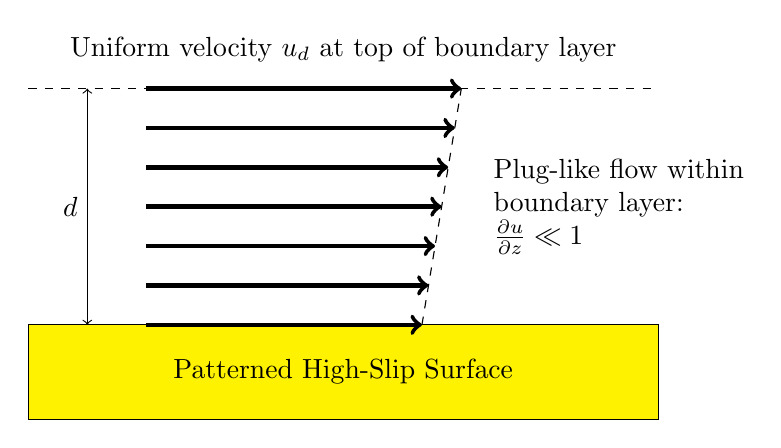
\begin{tikzpicture}
\draw[fill=yellow] (0,0) rectangle node{Patterned High-Slip Surface} (8,-1.2);
\draw[dashed] (0,3) -- ++(8,0);
\node at (4,3.5) {Uniform velocity $u_d$ at top of boundary layer};
\draw[<->] (0.75,0) -- node[left]{$d$} ++(0,3);

\foreach \z in {0,0.5,1,1.5,2,2.5,3}
    {\draw[->, ultra thick] (1.5,\z) -- ++(3.5 + \z/6,0);}
    
\draw[dashed] (5,0) -- ++(0.5,3);
    
\node at (7.5,1.5)[align=left] 
{Plug-like flow within\\ boundary layer:\\ $\frac{\partial u}{\partial z} \ll 1 $};
\end{tikzpicture}
\end{center}

\begin{center}
\begin{tikzpicture}
\draw (-1.5,0) -- (2.5,0);
\draw[->] (0,1) -- node[above]{$u_d$} ++(1.33,0);
\draw (0,0) -- node[left] {$d$} ++(0,1);
\draw[dashed] (0,0) -- node[left] {$b$} ++(0,-6);
\draw[dashed] (0,-6) -- (1.33,1);

\node at (2,-3) {$ \frac{\partial u}{\partial z} = \frac{u_d}{d+b}  $};
\end{tikzpicture}
\end{center}

Geometrically
\begin{equation}
\frac{\partial u}{\partial z} = \frac{u_d}{d+b} 
\end{equation}

In Appendix C we show that if the length scale of the surface pattern is fixed, then $d$ may scale as $u_d$.  In that case, the ratio $u_d/d$ is constant, while $b$ is variable. So:
\begin{equation}
\frac{u_d}{d+b} = \frac{\frac{u_d}{d}}{1 + \frac{b}{d}} \to 0 
\qquad \text{if} \qquad
\frac{b}{d} \to \infty
\qquad \text{if} \qquad
\frac{d}{b} \to 0
\end{equation}
Thus
\begin{equation}
\frac{\partial u}{\partial z} \ll 1 \qquad \text{if} \qquad\frac{d}{b} \ll 1
\end{equation}

Therefore let us concentrate on the worst case, where $b$ is minimal, and introduce the small parameter
\begin{equation}
\epsilon = \frac{d}{\bmin}, \qquad \epsilon \ll 1
\end{equation}
where $\bmin$ is the minimum slip length of the surface.

\subsubsection*{Perturbed Navier Slip}

The Navier slip condition relates the shear rate to the slip velocity.  With $\epsilon$, we can express the slip condition as a perturbation away from shear-free plug flow.  Multiplying both sides by $\epsilon$ gives:
\begin{equation}
\frac{d}{\bmin} b(x,y) \frac{\partial u }{\partial z} = \epsilon u(0)
\end{equation}
Define the normalised slip length:
\begin{equation}
\hat{b} = \frac{b(x,y)}{\bmin},   \qquad \hat{b} \geq 1
\end{equation}
So the perturbed slip condition is:
\begin{equation}
d \hat{b} \frac{\partial u}{\partial z} = \epsilon u(0)
\end{equation}


\subsubsection*{Perturbation Expansion}

The velocity solution to Stokes flow is assumed to be expressible as a power series in $\epsilon$:
\begin{equation}
\vec{u} = \vec{u}_0 + \epsilon \vec{u}_1 + O(\epsilon^2)
\end{equation}
where
\begin{equation}
\vec{u}_0 + \epsilon \vec{u}_1 = (u_0, v_0, w_0) + \epsilon(u_1, v_1, w_1)
\end{equation}
The pressure is similarly expressed as a power series in $\epsilon$:
\begin{equation}
p = p_0 + \epsilon p_1 + O(\epsilon^2)
\end{equation}

Both are inserted into the equations of Stokes flow with perturbed slip, giving to first order:

\begin{gather}
\nabla^2 \vec{u}_0 + \epsilon \nabla^2 \vec{u}_1 =
 \frac{1}{\mu} \nabla p_0 + \epsilon \frac{1}{\mu} \nabla p_1 \\
\nabla \cdot \vec{u}_0 + \epsilon \nabla \cdot \vec{u}_1 = 0  \\
p_0(x,y,z) + \epsilon p_1(x,y,z) = p_0(x+L,y,z) + \epsilon p_1(x+L,y,z) \\
u_0(x,y,d) + \epsilon u_1(x,y,d) = u_d \\ 
 d \hat{b} \frac{\partial u_0}{\partial z}  +
  \epsilon  d \hat{b} \frac{\partial u_1}{\partial z}
= \epsilon u_0
\end{gather}


\subsubsection*{Zeroth Order}

By construction, setting $\epsilon$ to zero gives shear-free flow:
\begin{gather}
\nabla^2 \vec{u}_0  = \frac{1}{\mu} \nabla p_0 \\
u_0(x,y,d) = u_d \\ 
\frac{\partial u_0}{\partial z} \rvert_{z=0} = 0
\end{gather}
whose solution is plug flow.  That is, $u_0(x,y,z) = u_d$, constant everywhere.

\subsection*{First Order}

Cancelling the zeroth order terms and dividing by $\epsilon$ gives the first order problem:
\begin{gather}
\nabla^2 \vec{u}_1 = \frac{1}{\mu} \nabla p_1 \\
\nabla \cdot \vec{u}_1 = 0  \\
p_1(x,y,z) = p_1(x+L,y,z) \\
u_1(x,y,d) = 0 \\ 
d \hat{b} \frac{\partial u_1}{\partial z} \rvert_{z=0} = u_0 =  u_d
\end{gather}

Note that the zeroth order solution appears in the slip condition.

\subsubsection*{Eliminate Pressure with Vorticity}

The standard way to eliminate the pressure is to use the vorticity $\nabla \times \vec{u}$.
Taking the curl of both sides of the Stokes equation gives:
\begin{equation}
\nabla \times \nabla^2 \vec{u}_1  = \nabla \times \frac{1}{\mu} \nabla p_1 
\end{equation}
The right hand side is identically zero, leaving $ \nabla \times \nabla^2 \vec{u}_1 = 0 $.
Recall that the vector Laplacian is:
\begin{equation}
\nabla^2 \vec{u}_1 = \left( \nabla^2 u_1, \nabla^2 v_1, \nabla^2 w_1 \right)
\end{equation}
so that $  \nabla \times \nabla^2 \vec{u}_1 = 0 $ is
\begin{equation}
\left( 
\frac{\partial}{\partial y} \nabla^2 w_1 - \frac{\partial}{\partial z} \nabla^2 v_1,
\frac{\partial}{\partial z} \nabla^2 u_1 - \frac{\partial}{\partial x} \nabla^2 w_1,
\frac{\partial}{\partial x} \nabla^2 v_1 - \frac{\partial}{\partial y} \nabla^2 u_1
\right) = (0,0,0)
\end{equation}

This gives three PDEs.  It turns out that the successfull strategy is to use the last two. Expanding out the Laplacian operator, these are:
\begin{gather}
\frac{\partial^3 u_1}{\partial z \partial x^2} + \frac{\partial^3 u_1}{\partial z \partial y^2}
+ \frac{\partial^3 u_1}{\partial z^3} =
\frac{\partial^3 w_1}{\partial x^3} + \frac{\partial^3 w_1}{\partial x \partial y^2}
+ \frac{\partial^3 w_1}{\partial x \partial z^2} 
\\
\frac{\partial^3 u_1}{\partial y \partial x^2} + \frac{\partial^3 u_1}{\partial y^3}
+ \frac{\partial^3 u_1}{\partial y \partial z^2} =
\frac{\partial^3 v_1}{\partial x^3} + \frac{\partial^3 v_1}{\partial x \partial y^2}
+ \frac{\partial^3 v_1}{\partial x \partial z^2} 
\end{gather}
It also happens that the successful strategy is to convert to last equation into an expression in $u_1$ and $w_1$.  We can do this because the incompressibility couples $u$, $v$ and $w$.  Specifically, the continuity equation $\nabla \cdot \vec{u}_1 = 0$ can be rearranged to:
\begin{equation}
\frac{\partial v_1}{\partial y} = - \frac{\partial u_1}{\partial x} - \frac{\partial w_1}{\partial z}
\end{equation}
To use this substitution, we first differentiate the last equation with respect to $y$:
\begin{equation}
\frac{\partial^4 u_1}{\partial y^2 \partial x^2} + \frac{\partial^4 u_1}{\partial y^4}
+ \frac{\partial^4 u_1}{\partial y^2 \partial z^2} =
\frac{\partial^4 v_1}{\partial y \partial x^3} + \frac{\partial^4 v_1}{\partial x \partial y^3}
+ \frac{\partial^4 v_1}{\partial x \partial y \partial z^2} 
\end{equation}
then make the substitution, giving:
\begin{multline}
\frac{\partial^4 u_1}{\partial y^2 \partial x^2} + \frac{\partial^4 u_1}{\partial y^4}
+ \frac{\partial^4 u_1}{\partial y^2 \partial z^2} =  \\
- \frac{\partial^3 }{\partial x^3}
 \left[ \frac{\partial u_1}{\partial x} + \frac{\partial w_1}{\partial z} \right] 
- \frac{\partial^3 }{\partial x \partial y^2}
 \left[ \frac{\partial u_1}{\partial x} + \frac{\partial w_1}{\partial z} \right] 
- \frac{\partial^3 }{\partial x \partial z^2}
 \left[ \frac{\partial u_1}{\partial x} + \frac{\partial w_1}{\partial z} \right]  
\end{multline}
%\begin{multline}
%\frac{\partial^4 u}{\partial y^2 \partial x^2} + \frac{\partial^4 u}{\partial y^4}
%+ \frac{\partial^4 u}{\partial y^2 \partial z^2} =  \\
%- \frac{\partial^4 u}{\partial x^4} - \frac{\partial^4 w}{\partial x^3 \partial z} 
%- \frac{\partial^4 u}{\partial x^2 \partial y^2} 
%      - \frac{\partial^4 w}{\partial x \partial y^2 \partial z} 
%- \frac{\partial^4 u}{\partial x^2 \partial z^2} 
%      - \frac{\partial^4 w}{\partial x \partial z^3} 
%\end{multline}
Simplified:
\begin{multline}
\frac{\partial^4 u_1}{\partial x^4} 
+ 2 \frac{\partial^4 u_1}{\partial x^2 \partial y^2} 
+ \frac{\partial^4 u_1}{\partial y^4}
+ \frac{\partial^4 u_1}{\partial x^2 \partial z^2} 
+ \frac{\partial^4 u_1}{\partial y^2 \partial z^2}
=  \\
- \frac{\partial^4 w_1}{\partial x^3 \partial z} 
- \frac{\partial^4 w_1}{\partial x \partial y^2 \partial z} 
- \frac{\partial^4 w_1}{\partial x \partial z^3} 
\end{multline}

Thus we have two PDEs in two variables, $u_1$ and $w_1$.
\begin{gather}
\frac{\partial^3 u_1}{\partial z \partial x^2} + \frac{\partial^3 u_1}{\partial z \partial y^2}
+ \frac{\partial^3 u_1}{\partial z^3} =
\frac{\partial^3 w_1}{\partial x^3} + \frac{\partial^3 w_1}{\partial x \partial y^2}
+ \frac{\partial^3 w_1}{\partial x \partial z^2} 
\\
\frac{\partial^4 u_1}{\partial x^4} 
+ 2 \frac{\partial^4 u_1}{\partial x^2 \partial y^2} 
+ \frac{\partial^4 u_1}{\partial y^4}
+ \frac{\partial^4 u_1}{\partial x^2 \partial z^2} 
+ \frac{\partial^4 u_1}{\partial y^2 \partial z^2}
=
- \frac{\partial^4 w_1}{\partial x^3 \partial z} 
- \frac{\partial^4 w_1}{\partial x \partial y^2 \partial z} 
- \frac{\partial^4 w_1}{\partial x \partial z^3} 
\end{gather}


\subsubsection*{Fourier Series}

Because the flow is periodic, it is natural to write $u_1$ as a Fourier series:
\begin{equation}
u_1(x,y,z) = \sum_{\vec{k}}^{\infty} U_{\vec{k}}(z) \exp(i \vec{k}\cdot \vec{r})
\end{equation}
where $\vec{r} = (x,y)$ and the wave vector $\vec{k}$ is a reciprocal lattice vector defined by integers $p$ and $q$:
\begin{equation}
\vec{k} = (m,n) = (2\pi p, 2\pi q), \qquad k^2 = m^2 + n^2
\end{equation}
The Fourier coefficient is:
\begin{equation}
U_{\vec{k}}(z) = \frac{1}{L^2} \int_0^L \int_0^L u(x,y,z) \exp(i \vec{k} \cdot \vec{r})
\;dxdy
\end{equation}
Similarly for $w_1$:
\begin{equation}
w_1(x,y,z) = \sum_{\vec{k}}^{\infty} W_{\vec{k}}(z) \exp(i \vec{k}\cdot \vec{r})
\end{equation}

The two Fourier expansions for velocity are inserted into the two PDEs.  At this point, resulting mess of algebra was tackled with the computer algebra package Maple.

At length, one has two expressions that are true for arbitrary $\vec{r} = (x,y)$.  As a consequence, the following two ODEs in $U$ and $W$ are true for all $\vec{k}$:
\begin{gather}
\frac{d^3 U}{dz^3} - k^2 \frac{d U}{dz} = i \left( \frac{d^2 W}{dz^2} - k^2 W \right) m 
\label{DE1} \\
k^2 \frac{d^2 U}{dz^2} - k^4 U = i \left( \frac{d^3 W}{dz^3} - k^2 \frac{dW}{dz} \right) m
\label{DE2}
\end{gather}
(The parameters $k$ and $m$ are of course not independent.)

\subsubsection*{Solving the DEs}

It turns out that a successful strategy is to solve for $W(z)$ first, then substitute the solution back into Equation (\ref{DE1}), allowing us to solve for $U(z)$.

\vspace{1em}
\textbf{Solve for $W(z)$}

After multiplying Equation (\ref{DE1}) by $k^2$, and  differentiating  Equation (\ref{DE2}) with respect to $z$, the two equations may be combined to:
\begin{equation}
\frac{d^4 W}{dz} - 2 k^2 \frac{d^2 W}{dz^2} + k^4 W = 0
\end{equation}
The general solution of which is:
\begin{equation}
W(z) = \left( P_{\vec{k}} + Q_{\vec{k}} z \right) e^{-kz} +
\left( R_{\vec{k}} + S_{\vec{k}} z \right) e^{kz}
\end{equation}

Now, at the top of the boundary layer, flow is defined to be in the $x$ direction only.  Therefore $w_1(x,y,d) = 0$, which requires that
\begin{equation}
W(d) = 0
\end{equation} 
The $e^{kz}$ term of $W(z)$ is obviously a problem, since $e^{kd}$ increases rapidly with increasing $d$.  Therefore we must have $R_{\vec{k}} = S_{\vec{k}} = 0$.

Furthermore, the bottom surface is impermeable, so $w_1(x,y,0) = 0$, which requires that $W(0) = 0$.  An immediate corollary is that $W(0) = P_{\vec{k}} = 0$.
We are left with:
\begin{equation}
W(z) = Q_{\vec{k}} z e^{-kz}
\end{equation} 


\textbf{Solving for $U(z)$}

We insert the solution for $W(z)$ into Equation (\ref{DE2}), yielding an ODE in $U(z)$:
\begin{equation}
\frac{d^3 U}{dz^3} - k^2 \frac{d U}{dz} = i Q_{\vec{k}} m k^2 e^{-kz} 
\end{equation}
For non-zero $k$, the general solution is:
\begin{equation}
U_{\vec{k}}(z) = \left( P_{\vec{k}} + i Q_{\vec{k}} \frac{m}{k^2} \right) e^{-kz}
+ B_{\vec{k}} e^{kz}
\end{equation}
For $k = 0$, the ODE reduces to:
\begin{equation}
\frac{d^3 U}{dz^3} = 0
\end{equation}
whose solution is:
\begin{equation}
U_0 = A_0 + B_0 z + C_0 z^2
\end{equation}


\textbf{Assemble $u_1(x,yz)$ solution}

We have found the Fourier coefficients in their most general form.  We now insert them into the Fourier series expression $ u_1(x,y,z) = \sum_{\vec{k}}^{\infty} U_{\vec{k}}(z) \exp(i \vec{k}\cdot \vec{r}) $:
\begin{gather}
u_1(x,y,z) = A_0 + B_0 z + C_0 z^2 + \sum_{k \neq 0} 
\left(  A_{\vec{k}} e^{-kz} + B_{\vec{k}} e^{kz} \right)
\exp(i \vec{k}\cdot \vec{r})\\
\text{where} \quad
A_{\vec{k}} = \left( P_{\vec{k}} + i Q_{\vec{k}} \frac{m}{k^2} \right)
\end{gather}

\textbf{Use periodicity to eliminate $C_0$}

Inserting our expression for $u_1(x,y,z)$ into the $x$ component of the Stokes equation:
\begin{equation}
\frac{\partial^2 u_1}{\partial x^2} + \frac{\partial^2 u_1}{\partial y^2} +
\frac{\partial^2 u_1}{\partial z^2} =
\frac{1}{\mu} \frac{\partial p_1}{\partial x}
\end{equation}
gives:
\begin{multline}
- m^2
\sum_{k \neq 0} 
\left(  A_{\vec{k}} e^{-kz} + B_{\vec{k}} e^{kz} \right)
\exp(i \vec{k}\cdot \vec{r})
- n^2
\sum_{k \neq 0} 
\left(  A_{\vec{k}} e^{-kz} + B_{\vec{k}} e^{kz} \right)
\exp(i \vec{k}\cdot \vec{r}) \\
+ 2 C_0
+ k^2
\sum_{k \neq 0} 
\left(  A_{\vec{k}} e^{-kz} + B_{\vec{k}} e^{kz} \right)
\exp(i \vec{k}\cdot \vec{r})
= \frac{1}{\mu} \frac{\partial p_1}{\partial x}
\end{multline}
Since $k^2 = m^2 + n^2$, this reduces to:
\begin{equation}
2 C_0 = \frac{1}{\mu} \frac{\partial p_1}{\partial x}
\end{equation}
Integrate this over one period:
\begin{gather}
\int_0^L 2 C_0 \;dx = \int_0^L \frac{1}{\mu} \frac{\partial p_1}{\partial x} \;dx \\
2 C_0 L = \frac{1}{\mu} [ p_1(L,y,z) - p_1(0,yz) ] = 0
\end{gather}
The flow is shear-driven only, so the pressure is periodic: $p_1(x,y,z) = p_1(x+L,y,z)$.  Therefore the right-hand side of the integral vanishes, and we are left with $C_0 = 0$.

\vspace{1em}
\textbf{Use top-of-boundary-layer condition to find $A_0$}

At the top of the boundary layer, the flow is (arbitrarily close to) uniform laminar flow with velocity $u_d$ in the $x$ direction only.  Above the boundary layer, the zeroth order solution is exact, so the first order term vanishes:
\begin{equation}
u_1(x,y,d) = 0
\end{equation} 
Inserting our expression gives:
\begin{equation}
A_0 + B_0 d + \sum_{k \neq 0} 
\left(  A_{\vec{k}} e^{-kd} + B_{\vec{k}} e^{kd} \right)
\exp(i \vec{k}\cdot \vec{r})
= 0
\end{equation}

The height $d$ of the boundary layer is essentially chosen to be large enough that the $u_1(x,y,d)$ term is arbitrarily small.  This works for the $e^{-kd}$ term; it can be made arbitrarily small with increasing $d$.  But the $B_{\vec{k}} e^{kd}$ term gets arbitrarily \emph{large} with increasing $d$.  Therefore, we require that $B_{\vec{k}} = 0$ for all $k \neq 0$.

Then the sum term is negligible, and we are left with:
\begin{equation}
A_0 + B_0 d = 0
\end{equation}
from which it follows that $A_0 = - B_0 d $.  Our first-order velocity term is now:
\begin{equation}
u_1(x,y,z) =  B_0 (z - d) + \sum_{k \neq 0} 
\left(  A_{\vec{k}} e^{-kz} \right)
\exp(i \vec{k}\cdot \vec{r})
\end{equation}

\textbf{Use Slip Boundary Condition to find $B_0$}

We have found that the Fourier coefficient for $\vec{k} = (0,0)$ is $U_0 = B_0 (z - d)$.
We may equate this with the formal definition:
\begin{equation}
U_0 = B_0 (z - d) = \frac{1}{L^2} \int_0^L \int_0^L u_1(x,y,z) \;dxdy
\end{equation}
and differentiate with respect to $z$:
\begin{equation}
\frac{d}{dz} ( B_0 z - B_0 d) = \frac{1}{L^2} \int_0^L \int_0^L \frac{d}{dz} u_1(x,y,z) \;dxdy
\end{equation}
then evaluate at $z=0$:
\begin{equation}
B_0 = \frac{1}{L^2} \int_0^L \int_0^L \frac{d u_1}{dz} \rvert_{z=0} \;dxdy
\end{equation}
At this point we can substitute the slip boundary condition:
\begin{equation}
\frac{d u_1}{d z} \rvert_{z=0} = \frac{1}{d \hat{b}} u_d
\end{equation}
to get:
\begin{equation}
B_0 = \frac{1}{L^2} \int_0^L \int_0^L \frac{1}{d \hat{b}} u_d \;dxdy
\end{equation}
The double integral is the area-weighted average:
\begin{equation}
B_0 = \frac{u_d}{d} \frac{1}{L^2} \int_0^L \int_0^L \frac{1}{\hat{b}} \;dxdy
= \frac{u_d}{d} \left< \frac{1}{\hat{b}} \right>
\end{equation}

\vspace{1em}
So the \textbf{first order velocity term} is:
\begin{equation}
u_1(x,y,z) =  \frac{u_d}{d} \left< \frac{1}{\hat{b}} \right> (z - d)
 + \sum_{k \neq 0} 
\left(  A_{\vec{k}} e^{-kz} \right)
\exp(i \vec{k}\cdot \vec{r})
\end{equation}


\subsubsection*{Bolt Together Velocity Solution}
We now have all the parts of the $x$ velocity perturbaton expansion $u(x,y,z) = u_0(x,y,z) + \epsilon u_1(x,y,z)$.  Bolting it together gives:

\begin{equation}
u(x,y,z) = u_d
 + \epsilon \frac{u_d}{d} \left< \frac{1}{\hat{b}} \right> (z - d)
 +  \epsilon \sum_{k \neq 0} 
\left(  A_{\vec{k}} e^{-kz} \right)
\exp(i \vec{k}\cdot \vec{r})
\end{equation}
Recall that:
\begin{equation}
\epsilon = \frac{d}{\bmin} \qquad \text{and} \qquad
\hat{b} = \frac{b}{\bmin}
\end{equation}
therefore:
\begin{equation}
\epsilon \frac{u_d}{d} \left< \frac{1}{\hat{b}} \right> 
= \frac{d}{\bmin} \frac{u_d}{d} \left< \frac{\bmin}{b} \right> 
= u_d \left< \frac{1}{b} \right>
\end{equation}

Thus, the final velocity solution is:
\begin{equation}
u(x,y,z) = u_d
 + u_d\left< \frac{1}{b} \right> (z - d)
 +  \epsilon \sum_{k \neq 0} 
\left(  A_{\vec{k}} e^{-kz} \right)
\exp(i \vec{k}\cdot \vec{r})
\end{equation}

\subsubsection*{Effective Slip Length}

Since we know the height $d$ of the boundary layer and the velocity $u_d$ at the top of the boundary layer, if we know the shear rate at top of the boundary layer, we can calculate the effective slip length.

The flow is uniform and laminar above the boundary layer, so simple shear obtains, and the shear rate is simply the velocity gradient $\frac{d}{dz} u$:
\begin{equation}
\frac{d}{dz} u(x,y,z) = 
 u_d\left< \frac{1}{b} \right>
 - \epsilon \sum_{k \neq 0} 
\left( k A_{\vec{k}} e^{-kz} \right)
\exp(i \vec{k}\cdot \vec{r})
\end{equation}
By construction, for $z$ at (and above) $d$, the $e^{-kz}$ term is negligible. So:
\begin{equation}
\frac{du}{dz} \rvert_{z=d} = u_d\left< \frac{1}{b} \right>
\end{equation}
Rearranging to the familiar form of Navier slip:
\begin{equation}
 u_d = \left< \frac{1}{b} \right>^{-1} \frac{du}{dz} \rvert_{z=d}
\end{equation}
This defines the effective slip length of a virtual surface \emph{at the top of the boundary layer:}
\begin{equation}
\beff = \left< \frac{1}{b} \right>^{-1}
\end{equation}
The true slip length of the \textbf{solid surface} is less by the thickness of the boundary layer:
\begin{equation}
\beff = \left< \frac{1}{b} \right>^{-1} - d
\end{equation}

Now, in the homogenization technique, we took the limit of the period of the surface patterning diminishing to zero.  This is equivalent to the limit of the thickness of the boundary layer diminishing to zero.  Therefore, the perturbed effective slip length reconciles with the homogenized slip length.
\begin{equation}
\lim_{d \to 0} \beff = \left< \frac{1}{b} \right>^{-1}
\end{equation}

\section*{Perturbed Couette Flow}

A similar analysis can be done for perturbed Couette flow.

In this case, flow is \emph{close to} Couette flow if the maximum slip length $\bmax$ of the surface is \emph{small} compared to the height $d$ of the boundary layer.  Therefore a suitable choice of perturbation parameter is:
\begin{equation}
\epsilon = \frac{\bmax}{d}
\end{equation} 
And the normalised slip length can be defined as:
\begin{equation}
\hat{b} = \frac{b(x,y)}{\bmax}, \qquad 0 \leq \hat{b} \leq 1
\end{equation}
Then both sides of the Navier slip condition can be divided by $\epsilon$:
\begin{equation}
\frac{1}{\epsilon} u(x,y,0) = \frac{d}{\bmax} b(x,y) \frac{\partial u}{\partial z} \rvert_{z=0}
\end{equation}
So the perturbed slip condition is:
\begin{equation}
u(x,y,0) = \epsilon d \hat{b} \frac{\partial u}{\partial z} \rvert_{z=0}
\end{equation}

As before, the velocity solution is written as a perturbation expansion:
\begin{equation}
\vec{u} = \vec{u}_0 + \epsilon \vec{u}_1 = (u_0, v_0, w_0) + \epsilon(u_1, v_1, w_1)
\end{equation}
which is inserted into the Stokes, continuity, and various boundary equations.

The only difference is of course the slip condition.  To first order in $\epsilon$:
\begin{equation}
u_0 + \epsilon u_1 = \epsilon d \hat{b} \frac{\partial u_0}{\partial z} \rvert_{z=0}
\end{equation}

\subsubsection*{Zeroth Order}

By construction, setting $\epsilon = 0$ gives classic Couette flow:
\begin{gather}
u_0(x,y,d) = u_d \\
u_0(x,y,0) = 0
\end{gather}
whose solution is a linear interpolation between the top and no-slip boundary conditions:
\begin{equation}
u_0(x,y,z) = \frac{u_d}{d} z
\end{equation}

\subsubsection*{First Order}
Cancelling the zeroth order terms and dividing by $\epsilon$ gives the first order slip condition:
\begin{gather}
u_1 = d \hat{b} \frac{\partial u_0}{\partial z} \rvert_{z=0}
= d \hat{b} \frac{u_d}{d} \\
u_1 = \hat{b} u_d
\end{gather}
Again, the zeroth order solution enters the slip condition.

\vspace{1em}
The analysis proceeds exactly as before, until the point where we solve for the coefficient $B_0$.
\vspace{1em}

\textbf{Use Slip Boundary Condition to find $B_0$}

We have found that the Fourier coefficient for $\vec{k} = (0,0)$ is $U_0 = B_0 (z - d)$.
We may equate this with the formal definition:
\begin{equation}
U_0 = B_0 (z - d) = \frac{1}{L^2} \int_0^L \int_0^L u_1(x,y,z) \;dxdy
\end{equation}
If we evaluate this at $z=0$, we may substitute the first order slip condition:
\begin{equation}
- B_0 d = \frac{1}{L^2} \int_0^L \int_0^L \hat{b} u_d \;dxdy
\end{equation}

The double integral is the area-weighted average:
\begin{equation}
B_0 = - \frac{u_d}{d} \frac{1}{L^2} \int_0^L \int_0^L \hat{b} \;dxdy
= - \frac{u_d}{d} \left< \hat{b} \right>
\end{equation}

\vspace{1em}
So the \textbf{first order velocity term} is:
\begin{equation}
u_1(x,y,z) =  \frac{u_d}{d} \left< \hat{b} \right> (d - z)
 + \sum_{k \neq 0} 
\left(  A_{\vec{k}} e^{-kz} \right)
\exp(i \vec{k}\cdot \vec{r})
\end{equation}

\subsubsection*{Bolt Together Velocity Solution}
We now have all the parts of the $x$ velocity perturbaton expansion $u(x,y,z) = u_0(x,y,z) + \epsilon u_1(x,y,z)$.  Bolting it together gives:

\begin{equation}
u(x,y,z) = \frac{u_d}{d} z
 + \epsilon \frac{u_d}{d} \left< \hat{b} \right> (d - z)
 +  \epsilon \sum_{k \neq 0} 
\left(  A_{\vec{k}} e^{-kz} \right)
\exp(i \vec{k}\cdot \vec{r})
\end{equation}
Recall that:
\begin{equation}
\epsilon = \frac{\bmax}{d} \qquad \text{and} \qquad
\hat{b} = \frac{b}{\bmax}
\end{equation}
therefore:
\begin{equation}
\epsilon \frac{u_d}{d} \left< \hat{b} \right> 
= \frac{\bmax}{d} \frac{u_d}{d} \left< \frac{b}{\bmax} \right> 
= \frac{u_d}{d^2} \left< b \right>
\end{equation}
so that:
\begin{equation}
\epsilon \frac{u_d}{d} \left< \hat{b} \right> (d - z)
= \frac{u_d}{d} \left< b \right> - \frac{u_d}{d^2} \left< b \right> z
\end{equation}


Thus, the final velocity solution is:
\begin{equation}
u(x,y,z) = \frac{u_d}{d} 
\left[ z \left( 1 - \frac{\left< b \right>}{d} \right) + \left< b \right> \right]
 +  \epsilon \sum_{k \neq 0} 
\left(  A_{\vec{k}} e^{-kz} \right)
\exp(i \vec{k}\cdot \vec{r})
\end{equation}



\subsection*{Effective Slip Length}

As before, we calculate the effective slip length with the velocity gradient:
\begin{equation}
\frac{\partial}{\partial z} u(x,y,z) = \frac{u_d}{d} 
\left( 1 - \frac{\left< b \right>}{d} \right)
- \epsilon \sum_{k \neq 0} 
\left( k A_{\vec{k}} e^{-kz} \right)
\exp(i \vec{k}\cdot \vec{r})
\end{equation}
At $z$ greater than $d$, the $e^{-kz}$ term renders the sum term negligible, leaving:
\begin{equation}
\frac{\partial}{\partial z} u(x,y,z) = \frac{u_d}{d} 
\left( 1 - \frac{\left< b \right>}{d} \right)
\end{equation}
Rearranging to the form of Navier slip:
\begin{equation}
u_d = d \left( 1 - \frac{\left< b \right>}{d} \right)^{-1}
 \frac{\partial u}{\partial z} \rvert_{z=0}
\end{equation}
Implying an effective slip length at the top of the boundary of:
\begin{equation}
\beff = d \left( 1 - \frac{\left< b \right>}{d} \right)^{-1} 
= \frac{d}{1 - \frac{\left< b \right>}{d}}
\end{equation}

The slip length of the surface is found by subtracting $d$ from this:
\begin{gather}
\beff = \frac{d}{1 - \frac{\left< b \right>}{d}} - d \\
= \frac{d - d \left[ 1 - \frac{\left< b \right>}{d} \right]}{1 - \frac{\left< b \right>}{d}}
= \frac{ d - d + \left< b \right> }{1 - \frac{\left< b \right>}{d}} 
= \frac{\left< b \right> }{1 - \frac{\left< b \right>}{d}}
\end{gather}
We have assumed that for Couette-like flow, $\bmax \ll d$, therefore $ \left< b \right> \ll d$, and so $\left< b \right> / d$ is negligible.  We are left with:
\begin{equation}
\beff = \left< b \right>
\end{equation}

\subsection*{Conclusion}

The effective slip length found by perturbative methods reconciles with the effective slip length found by homogenization (for the case where the minimum slip length is large compared to the boundary layer thickness).  Because homogenization can deal with a non-flat surface, the homogenized effective slip length \emph{subsumes} the perturbative slip length.

In addition, the perturbative method can yield an effective slip length for the opposite case -- where the slip lengths are \emph{small} compared to surface length scales.

%\begin{center} \vspace{3em} \Coffeecup \end{center}

\bibliography{Lund_Thesis.bib}
\bibliographystyle{plain}

\end{document}

